\chapter{Outlook}
The next step is to implement the study setup, but still, there are some parameters to refine on. This takes place in the master's project. In this part, the technology and algorithms will be in the main focus. For technology, VR HMD will be compared and a decision will be made. Similar to motion tracking technologies. After this, algorithms for comparing two movements will be evaluated. When decisions are made, the implementation of the system will start. Eventually, a pilot testing session will take place followed by further refinements.
The milestones for the master's project are:
\begin{itemize}
\item Hardware requirements: 17.1.2020
\item Software Requirements: 24.1.2020
\item Implementation Start: 27.1.2020
\item Pilot Study: 2.3.2020
\item Refinements Implementation: 13.3.2020
\item Master’s Project Presentation and Report: 23.3.2020
\end{itemize}
The thesis will follow in the summer semester 2020. The results are planned to be published at a conference in 2020, compare figure~\ref{fig:outlook}.\\
For the master's thesis, a study will be conducted. The study will generate data suitable to answer the research question. This data will be analysed in detail and eventually be used to answer the research question.

\begin{figure}
	\centering
	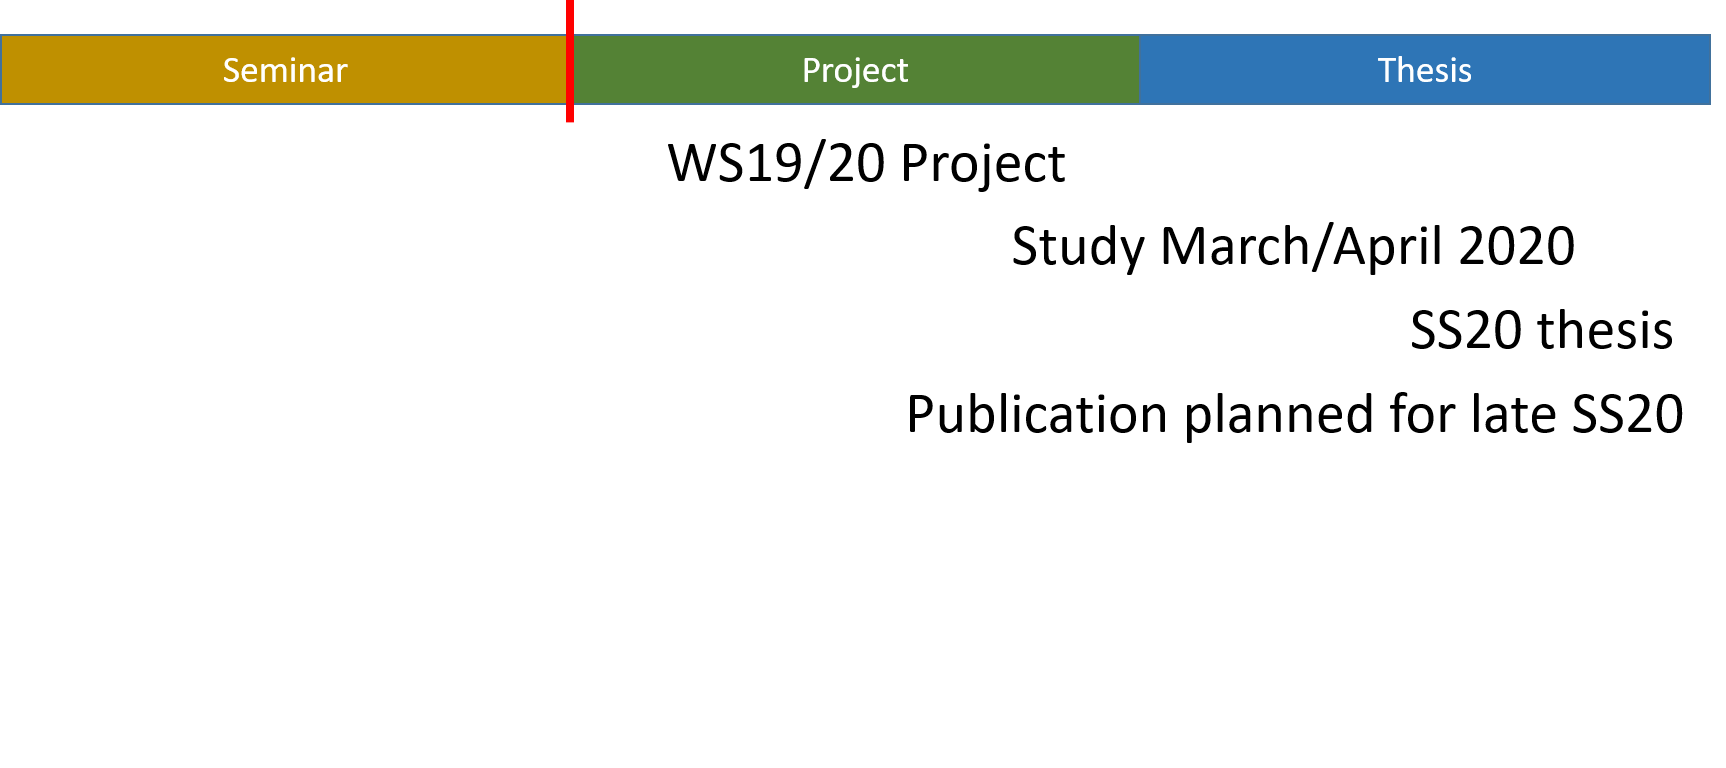
\includegraphics[width=1.0\textwidth]{img/outlook.png}
	\caption{Timetable for the master's thesis.}
	\label{fig:outlook}
\end{figure}